\section{Analyzing High-Dimensional Gene Expression Profiles}\label{sec:geneticData}

% Cells, DNA and RNA Stuff -> Dogma etc
The human genome, i.e.\ the entirety of genetic information that is stored in the form of 23 chromosome
pairs within every cell's nucleus, consists of about three billion base pairs of nucleic acids~\citep{venter}.
These base pairs are encoded in 20,000 to 25,000 genes that are defined as sections of the deoxyribonucleic acid (DNA).

In order to produce proteins, the genetic information of the DNA is first duplicated, then transcribed
into ribonucleic acid (RNA), more precisely into messenger RNA (mRNA), and subsequently translated into proteins, where it then defines
the protein's characteristics~\citep{crick, koonin}.
The central dogma of molecular biology by~\cite{crick} states that this process, also known as protein biosynthesis, cannot be reversed.
Therefore genetic information is `trapped' in the form of a protein's amino acids, once it is successfully
translated, without the chance of being re-translated into nucleic acids ever again~\citep{crick, koonin}.

While the genes in DNA consist of intron and extron sections, when transcribing, only the exons are kept
and then joined into one long RNA sequence in a process called `splicing'~\citep{wang10}.
The entirety of RNA molecules is then called transcriptome, as it is the ensemble of all RNA transcripts~\citep{malone, venter}.
These transcriptomes are dynamic, in contrast to the static genome~\citep{marguerat}
and provide valuable data on gene expressions, i.e.\ on the genetic and epigenetic characteristics of the cell~\citep{wang09, jones}.

% Genetics and Epigenetics
While the study of genetics addresses the inherited sequence of genes in the genome, epigenetics
focus on the extent, to what the individual genes are activated or deactivated within a specific cell~\citep{jones,jaenisch}.
These distinct gene expressions are influenced by the environment and are
also partially heritable, even though no DNA mutation is involved~\citep{jaenisch}.
A human has an explicit genome that is usually the same in every cell,
whereas the epigenome is in general different for distinct cell types, like liver and pancreas cells,
leading to cell types with different characteristics and functions.

% Cancer research questions -> Why do I want to analyze gene expressions?
Both, genetic and epigenetic, abnormalities are responsible for cancer development at all stages~\citep{jones, jaenisch}. % -> modified gene expressions
One of the main goals of medical oncology is therefore to discover novel genes that are differentially expressed by cancerous and benign cells~\citep{guo13},
or even by different subtypes of cancer.
This can be done by profiling the cell's gene expressions and measuring the differences in gene expression levels between sample classes.
The striking genes potentially produce tumor promoting or suppressing proteins and could therefore be possible starting points for improved cancer treatments.

In the following sections the modified SCM algorithm with data-dependent rays as 
base classifiers is used within a \(10 \times 10\) cross-validation to execute such an analysis on some
extremely high dimensional gene expression data sets, in order to detect compact classification
rules and therefore identify small sets of significant genes.

%%%%%%%%%%%%%%%%%%%%%%%%%%%%%%%%%%%%%%%%%%%%%%%%%%%%%%%%%%%%%%%%%%%%%%%%%%%%%%%%%%%%%%%%%%%%

\subsection{Methods to Quantify, Analyze and Compare Gene Expressions}

% How to analyze gene expressions?
To conduct quantitative analysis of gene expressions, the transcriptome needs to be characterized
by measuring the concentrations of all transcripts that are present at the given time.
This is usually done either by applying microarrays or RNA sequencing, also known as `RNA-seq',
the two most popular high-throughput technologies for gene expression profiling~\citep{li09,guo13}.
Both methods usually result in very similar outcomes~\citep{guo13}, however the two approaches
still have some differences.

% Microarrays and their problems
Microarrays, introduced in~\cite{schena}, are one of the first approaches for the analysis of transcriptomes~\citep{malone}.
Here RNA probes are extracted from samples of two different classes, like benign and cancerous cells, and reverse transcribed into complementary DNA (cDNA).
These cDNAs are then labeled using fluorescent dyes, placed on microarray chips and scanned~\citep{malone}.
A position on the chip will now become discolored, if the gene of this spot is expressed in one of the samples.
This allows comparisons of the expression of each gene in both sample classes.

This technology was especially popular till the 2010s~\citep{guo13} and well established for a long period of time,
leading to a lot of existing research and well assessed standards~\citep{malone}.
However with the introduction of RNA-seq by~\cite{wang09} and the increasing availability
of extremely high-throughput methods to process genetic data, microarrays lost a lot of their popularity~\citep{malone, li09}.

% RNA-seq
RNA-seq accurately estimates gene expression levels by utilizing next-generation sequencing (NGS)~\citep{guo13}.
There are different sequencers available. In the following I will focus in the `Illumina' sequencing protocol of~\cite{wang09}.
To prepare the sequencing library, an extracted RNA probe is broken down into small fragments of about 200 to 300 base pairs each,
which are then re-transcribed into cDNA~\citep{marguerat, wang09}.
These fragments are called `reads'.
The short sequence reads can now be aligned with the reference genome of a sample~\citep{li09}.
Thanks to NGS and its parallel processing, this sequencing process has a very high-throughput~\citep{franchis}.
Yet, reads do not have a 100\% accuracy rate and small errors in mapping happen regularly.
The number of reads that are mapped to a certain gene,also known as the `raw count' of a gene~\citep{li11}, now
estimates the gene expression level of the according gene in the sample~\citep{marguerat, wang09}.

% Normalizations for RNA-seq data
These raw counts may however vary from gene to gene and from sample to sample, as
samples and reads may be of different qualities, depths and lengths~\citep{li11, zhao, guo13}.
In order to ensure the comparability of various sample's gene expressions, these factors of irregularity
need to be offset to the highest possible extent.
This process of normalization then enables the actual estimated quantification of the gene expression levels~\citep{zhao}.

% RSEM
One possibility to estimate gene expression levels, is to use the RNA-seq by expectation maximization (RSEM) software library by~\cite{li11}.
This framework computes an accurate quantification of transcripts even for use cases without a reference genome.
In an RNA-seq reads may map to multiple positions in the reference genome,
usually to isoforms, i.e.\ slightly different versions of the same gene, or splicing junctions~\citep{li09}.
This problem is often solved by simply discarding and reads that have such multiple mappings,
however RSEM instead uses an expectation maximization algorithm that estimates the
true origin of a multi-read expression~\citep{li11}.

% TPM, FPKM, RPKM
The RSEM algorithm then usually returns the resulting expected counts in a transcripts per million (TPM) normalization,
meaning that the counts are first divided by the gene's length in kilobit and subsequently
by the total number of reads that are mapped to this sample \(\times 10^{-6}\)~\citep{zhao, li11}.
This ensures an even scaling of the estimated counts, regarding the gene length, as well as the sequencing depth, and
therefore offsets the transcript's abundances.
Other popular normalizations for RNA-seq data like reads per kilobase million (RPKM) and fragments per kilobase million (FPKM) are not supported by the RSEM library~\citep{li11}.
Those approaches are based on the same two normalization steps as TPM, however this time in a reversed order.
More information on them can be found in~\cite{zhao}.

% final comparison microarray and RNA-seq
Until today an analysis by microarrays is cheaper to realize than one by RNA-seq,
as a huge amount of genes can be processed simultaneously
and even multiple RNA probes can be examined on the same chip~\citep{guo13}.
Additionally the resulting data of a microarray analysis is much more compact and therefore cheaper to store~\citep{malone}.
Yet, RNA-seq is able to analyze the transcriptome's fine structure more precisely, as it `provides direkt access to the sequence'~\citep[p.35]{malone}.
It can detect differences even between extremely similar expressions and examine structural invariants of genes like
splicing junctions~\citep{guo13, malone, wang09}.
Furthermore the limitation of microarrays, that only expressions of predefined genes can
be detected, does not exist for RNA-seq analysis~\citep{guo13, malone}.

%%%%%%%%%%%%%%%%%%%%%%%%%%%%%%%%%%%%%%%%%%%%%%%%%%%%%%%%%%%%%%%%%%%%%%%%%%%%%%%%%%%%%%%%%%%%
\subsection{Origin and Specification of the Employed Data Sets}

% TCGA
In the following, various RNA-seq data sets from the cancer genome atlas (TCGA)~\citep{tcga08} are analyzed.
The TCGA is a huge, publicly available, research data base, founded by the U.S. government and implemented by the National Cancer Institute (NCI),
along with other institutions that can be found in~\cite{weinstein}.
It stores genomic data on over 30 different subtypes of human cancer on various body tissues~\citep{weinstein, guo13}.
Besides the gene expression profiles, each data set also contains much more information, such as the raw genetic data, the tumor's stage and details about the patient's background.
However, the analysis will focus on the RNA-seq data and not utilize these additional data tracks.

% Representative cancer data?
As for every scientific study, it is important that the samples, in this case the patients, are picked in a representative way,
in order for the study's results to be universally applicable.
Yet, besides the fact that the study solely considers U.S. citizens, according to~\cite{wang18}, the sample patients in the
TCGA data sets slightly differ from the average U.S. cancer patients, as they are on average younger and some ethnic backgrounds are over represented in certain data sets.
Furthermore all TCGA data sets tend to observe cancerous tissues at especially early stages, compared to the actual average stages
of tumors at the time of the initial diagnosis~\citep{wang18}.
But after all, these deviations are not too heavy and are largely due to the small sample sizes,
that are often a vital concern in medical genetic studies.
Therefore, I, just like many other researchers, still consider the TCGA studies to be representative enough for further consideration.

\begin{table}[ht]
        \centering
        \caption{Overview of the used TCGA cancer data sets and their abbreviations.}\label{tab:cancerTypes}
        \begin{tabular}{ll}
            \toprule
            tumor type & abbreviation \\
            \midrule
            KICH & Kidney Chromophobe \\
            KIRP & Kidney Renal Papillary Cell Carcinoma \\
            KIRC & Kidney Renal Clear Cell Carcinoma \\
            CHOL & Cholangiocarcinoma \\
            PAAD & Pancreatic Adenocarcinoma \\
            LIHC & Liver Hepatocellular Carcinoma \\
            COAD & Colon Adenocarcinoma \\ 
            READ & Rectum Adenocarcinoma \\ 
            \bottomrule
        \end{tabular}
\end{table}

% What classes I am comparing
As the TCGA data sets usually contain only very few gene samples of non-cancerous cells~\citep{guo13},
I will try the approach of not comparing healthy and malignant samples, but instead the gene expressions of eight
different cancer subtypes, illustrated in \autoref{tab:cancerTypes}.
The overall motivation is now to spot the genetic differences between the transcriptomes
of cells that are infected with the different tumor types,
in order learn about potential tumor causes.

\begin{table}[ht]
        \centering
        \caption{Overview of the analyzed RNA-seq data sets including the sample quantities within their classes.}\label{tab:geneData}
        \begin{tabular}{lllll}
            \toprule
            data set & class 0 & class 1 & |feat.| & |unique feat.| \\
            \midrule
            TCGA\_KICH\_vs\_KIRC & KICH (91) & KIRC (606) & 20,655 & 19,683 \\
            TCGA\_KICH\_vs\_KIRP & KICH (91) & KIRP (323) & 20,632 & 19,663 \\
            TCGA\_KIRP\_vs\_KIRC & KIRP (323) & KIRC (606) & 20,684 & 19,696 \\
            TCGA\_CHOL\_vs\_LIHC & CHOL (45) & LIHC (434) & 20,605 & 19,613 \\
            TCGA\_CHOL\_vs\_PAAD & CHOL (45) & PAAD (183) & 20,439 & 19,535 \\
            TCGA\_LIHC\_vs\_PAAD & LIHC (424) & PAAD (183) & 20,657 & 19,659 \\
            TCGA\_COAD\_vs\_READ & COAD (328) & READ (105) & 20,482 & 19,540 \\
            \bottomrule
        \end{tabular}
\end{table}

% seven data sets for the eight cancer types
Those sample sets are logically divided by the affected tissue type into two groups of three and one group of two cancer types.
Within the groups the types are then compared to each other, resulting in the seven
data sets displayed in \autoref{tab:geneData}, that can now be analyzed using the SCM's binary classification algorithm.

% How were these data sets generated/ preprocessed?
To be exact, this thesis uses the RNA-seq data sets that were preprocessed by~\cite{lausser20}.
They originally took the TCGA data sets from the genomic data commons (GDC) portal of the NCI.\
Here the gene expressions are quantified using a linear RSEM transformation with the `Illumina HiSeq' sequencing protocol.
Additionally, reads that are mapped on splice junctions are detected and properly aligned by the MapSplice algorithm of~\cite{wang10}.
~\cite{lausser20} then used the R library `\texttt{TCGAbiolinks}' to extract the sample's estimated counts,
along with their class labels, IDs and additional information, such as the feature names, from the GDC data sets into a matrix.

% Specifications
Each data set eventually consists of multiple samples from two different, but somewhat similar, cancer subtypes.
As typical for biomedical data, most classes each only contain a few dozen to a few hundred samples,
yet some, very common, cancer types, like the kidney renal clear cell carcinoma, have more samples provided.
The features are determined by the the about 20,000 genes of the human genome that are further specified by the gene symbol, as well as the gene ID, to tell apart isoforms and
genes that are placed distributed on multiple positions within a chromosome.
The values in the gene-sample matrix are thus the RSEM normalized estimated counts.

% Transparent preprocessing by me
A Julia routine, portrayed in \autoref{julia:loadRData}, was implemented for the just in time processing of the data sets of~\cite{lausser20}.
The algorithm is able to extract and convert the valuable data from the R data sets in a transparent and reliably way that works to such an extend,
that no prior preparation of the RNA-seq data is needed.
It extracts the gene-sample matrix, assigns the features their proper gene names and the samples their proper class labels.
Furthermore it discards duplicate features that have not only the same gene symbol and gene ID, but also the exact same vector of sample values.
Since those duplicates make up about 5\% of all features (see \autoref{tab:geneData}), their filtering speeds up the algorithm by quite some time
and prevents some illegal algorithm results.
In case of duplicate genes with the same gene identifier, but different sample vectors, the routine would
return an error message and terminate, however this is not the case for any of the relevant data sets.

%%%%%%%%%%%%%%%%%%%%%%%%%%%%%%%%%%%%%%%%%%%%%%%%%%%%%%%%%%%%%%%%%%%%%%%%%%%%%%%%%%%%%%%%%%%%
\subsection{Adjusting my SCM}\label{subsec:studySCM}

One has to keep in mind, that all the experiments are conducted by a cross-validation that is at least partially influenced by randomness.
Slight variations in the results are therefore completely normal and an accuracy of for example 0.926 instead of 0.927
does not necessarily mean, that one algorithm is inferior to the other.

% Adjusting the Minimum Conjunction Size
First of all the \(SCM_{DNF}\) was tested on the seven RNA-seq data sets with different values for
the \(minConjSize\) hyper-parameter.
The results, displayed in \autoref{tab:geneMCS}, reflect that the accuracies are optimal in
configurations with minimum conjunction sizes that prohibit extremely small conjunctions of only
a few data points, yet still allow conjunctions in the DNF that cover at least about 5\% of all, so far uncovered, samples.
This leads to the need of a well balanced \(minConjSize\) somewhere in the middle ground.
Additionally the classifiers in general become sparser with higher \(minConjSize\) values.
In the end, I decided on an optimal \(minConjSize\) of 10, as this parameter setting not only
ensures reasonable accuracies on all data sets, but also compact classification rules with only
comparatively few rays.

% Adjusting the Penalty Value \(p\)
Next, different configurations for the penalty value \(p\) were tested (see \autoref{tab:geneP}).
Since the data sets have very different rations of class 0 to class 1 samples, as depicted in \autoref{tab:geneData},
the optimal \(p\) value depends on the individual data set and its class balance.
Data sets with more class 0 samples perform visible better on low values for \(p\), while
sets with the majority of samples being of class 1 have better results using high \(p\).
Additionally the accuracies and the ratios of sensitivity and specificity
in the case of \(p=\frac{|\text{`negative samples'}|}{|\text{`positive samples'}|}\) were evaluated.
The results confirmed the hypothesis, that this configuration in general does not maximize
the SCM's accuracy, but usually offsets sensitivity and specificity quite well, as presented in \autoref{tab:genePMiddle}.
However \(p=1\) results in reasonable accuracies for all data sets.
The only exception here is \texttt{TCGA\_COAD\_vs\_READ} with an accuracy of only 0.761/0.753.
Its accuracy seems to be improvable with the use of even higher \(p\) values,
yet in fact this also never leads to accuracies higher than 0.8 and in the end only
converges to the baseline of \(\frac{328}{328+105} = 0.757\).

% Studying Ties
In \autoref{tab:geneTies} an \(SCM_{DNF}\) that utilizes ties as suggested in \autoref{sec:ties}, is compared to one that does not utilize them.
This study again showcases that the utilization of ties is not necessarily helpful.
While the algorithm without ties usually results in slightly higher accuracies, the routine with ties
in general returns more compact classification rules.
Yet, when looking at the amount of ties that were actually successfully utilized,
it becomes clear that the algorithm only detects a tie, that is not classified as useless, in about every tenth SCM execution.
However this is not caused by too few existing ties --- in fact there are hundreds to thousands of ties identified per SCM execution,
leading to the increased execution time and RAM demand of the algorithm ---
but by the fact, that the vast majority of ties leads to no improvement of the classifier and
therefore the attempt to utilize a tie ends in the algorithm's termination.
Thus, the differences in accuracy and number of used rays, between the two SCM versions,
are for six out of seven data sets mainly due to this earlier algorithm termination, but
not the actual successful use of a tie situation.
Hence, the utilization of ties is waived.

%%%%%%%%%%%%%%%%%%%%%%%%%%%%%%%%%%%%%%%%%%%%%%%%%%%%%%%%%%%%%%%%%%%%%%%%%%%%%%%%%%%%%%%%%%%%
\subsection{Biomedical Analysis}

\begin{figure}
        \centering
        \begin{subfigure}{\textwidth}
                \centering
                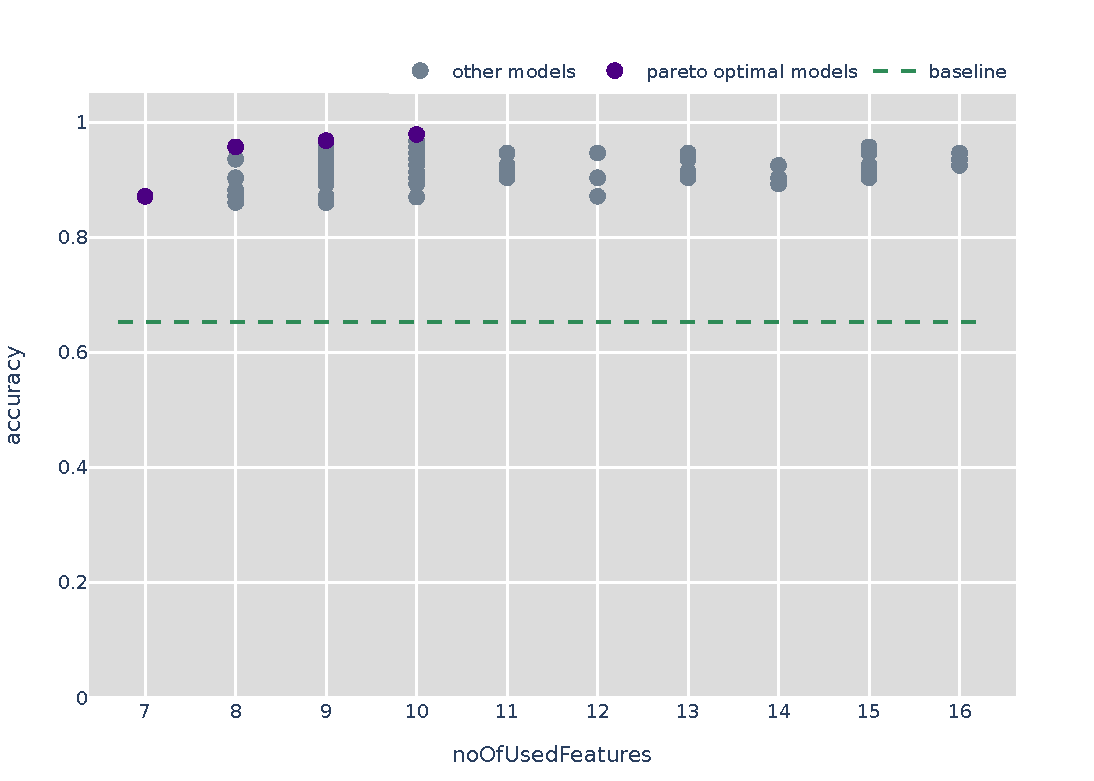
\includegraphics[width=0.85\columnwidth]{figures/genes/paretoFront_TCGA_KIRP_vs_KIRC.pdf}
                \caption{`TCGA\_KIRP\_vs\_KIRC' data set.}\label{fig:paretoKIRPvsKIRC}
        \end{subfigure}
        \hfill
        \begin{subfigure}{\textwidth}
                \centering
                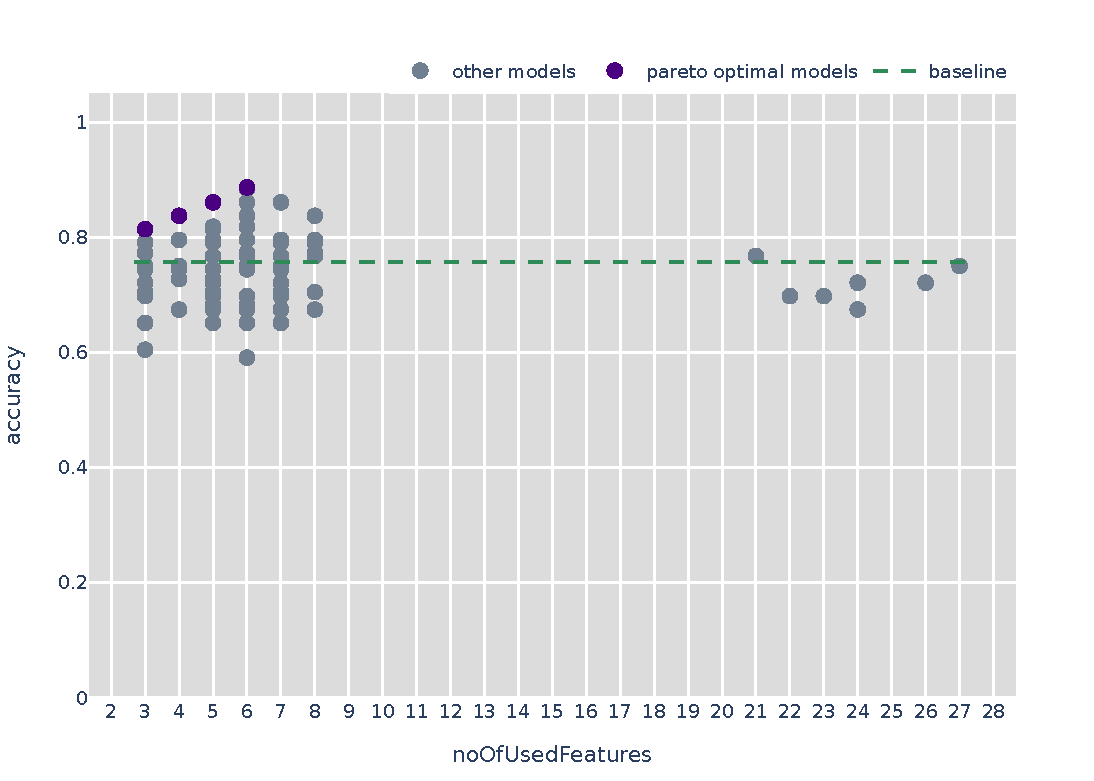
\includegraphics[width=0.85\columnwidth]{figures/genes/paretoFront_TCGA_COAD_vs_READ.pdf}
                \caption{`TCGA\_COAD\_vs\_READ' data set.}\label{fig:paretoCOADvsREAD}
        \end{subfigure}
        \caption{Accuracy-compactness plot for the cross-validation folds of two different RNA-seq data set.}\label{fig:genePareto}
\end{figure}

The resulting \(SCM_{DNF}\) configuration with \(p=1\) and \(minConjSize=10\) was now once more applied to the RNA-seq data sets.
This version of the SCM successfully creates very sparse classifiers (see \autoref{tab:geneCompact}) with in general high accuracies, way above the data's baselines, like visualized on
the example of `TCGA\_KIRP\_vs\_KIRC' in \autoref{fig:paretoKIRPvsKIRC}.
The only exception to this is the `TCGA\_COAD\_vs\_READ' data set, as illustrated in \autoref{fig:paretoCOADvsREAD}, where only the accuracies of 46.3\% of all
classifiers are actually above the baseline.
While the SCM is still able to classify the test samples with a reasonable accuracy through decision rules like
`\texttt{IF (EPHA3|2042 > 666.5 AND ADORA2B|136 > 305.5 AND ACO1|48 > 2297.5) OR (ELAVL2|1993 > 209 AND DDC|1644\\< 5461.5 AND ABCA4|24 < 8.5) THEN class `Rectum Adenocarcinoma'}',
it generally fails to a provide good classifications on unknown training samples.
I assume this is because of the high similarity of the two classes, as the examined tumors are both adenocarcinomas
and even located in similar, adjacent tissues.

\begin{table}[ht]
        \centering
        \caption{Summary of differentially expressed genes in the RNA-seq data sets.}\label{tab:geneGene}
        \begin{tabular}{lll}
                \toprule
                data set & class & comparatively high expressed genes \\
                \midrule
                \multirow{2}{*}{KICH\_vs\_KIRC} & KICH & NDUFS7 \\
                & KIRC & RPL39, MALAT1, ACO1 \\
                \specialrule{0pt}{0.8pc}{0pc}
                \multirow{2}{*}{KICH\_vs\_KIRP} & KICH & STAP1, ATP6V0D2, CLCNKB, ARMC4  \\
                & KIRP & CACNA1E, FZD4 \\
                \specialrule{0pt}{0.8pc}{0pc}
                \multirow{2}{*}{KIRP\_vs\_KIRC} & KIRP & FLRT3, GPS1, ACCN3, ATG2A, FGFR3 \\
                & KIRC & ELTD1, PHKA2, BNC1, CAPZA2, BMI1 \\
                \specialrule{0pt}{0.8pc}{0pc}
                \multirow{2}{*}{CHOL\_vs\_LIHC} & CHOL & CAPN6 \\
                & LIHC & APOE, MEA1, CDKN2D \\
                \specialrule{0pt}{0.8pc}{0pc}
                \multirow{2}{*}{CHOL\_vs\_PAAD} & CHOL & ASGR2, ACADM \\
                & PAAD & PTPRN \\
                \specialrule{0pt}{0.8pc}{0pc}
                \multirow{2}{*}{LIHC\_vs\_PAAD} & LIHC & ALDH4A1 \\
                & PAAD & EDN3 \\
                \specialrule{0pt}{0.8pc}{0pc}
                \multirow{2}{*}{COAD\_vs\_READ} & COAD & / \\
                & READ & EPHA3, ADORA2B, ACO1, ELAVL2, HOXD12 \\
                \bottomrule
        \end{tabular}
\end{table}

% Interpretation of the Results - WHAT DOES IT ALL MEAN?
To identify mutated genes, the feature histograms \autoref{fig:histKICHvsKIRC} to \autoref{fig:histCOADvsREAD},
the ray histograms, the constructed pareto-optimal classification rules, as well as the classifiers that are obtained when using all samples for training,
can be assessed.
In \autoref{tab:geneGene} all genes that each occur in at least
one histogram and additionally in at least one of the just mentioned classification rules are aggregated.
Hence, these genes are classified as relevant and sorted them in to their according classes, using the classifiers and ray histograms.

% 1. What do the genes mean? -> look for sth like "Patients who have pancreatic ductal adenocarcinoma show an overexpression of A1BG in pancreatic juice.[6]"
% 2. What do the numbers mean? Is 100 much? What does it mean? Maybe: What's the normal value? -- normalized number of reads that were successfully mapped to this gene
This analysis of the RNA-seq gene expressions revealed some genes, like \texttt{ATP6V0D2} and \texttt{CLCNKB}, that are actually known for being present in striking levels
in those corresponding cancer subtypes~\citep{zhou}.
However the vast majority of the significant gene expressions are actually not really associated to these specific cancer subtypes by prior research.
This results in my conclusion, that genes with very differential expressions in cancerous and benign cells, like the ones listed by~\cite{tcga13},
are usually not the ones that are identified as significant when comparing different, yet still quite similar, cancer subtypes.
Therefore I do in fact not classify the found genes to be extremely cancer promoting, but instead
to be those genes, that make up a tumor's subtleties.